\chapter{Performance Results}

\section{Data Layout Impact: AoS vs SoA}

\begin{figure}[h]
\centering
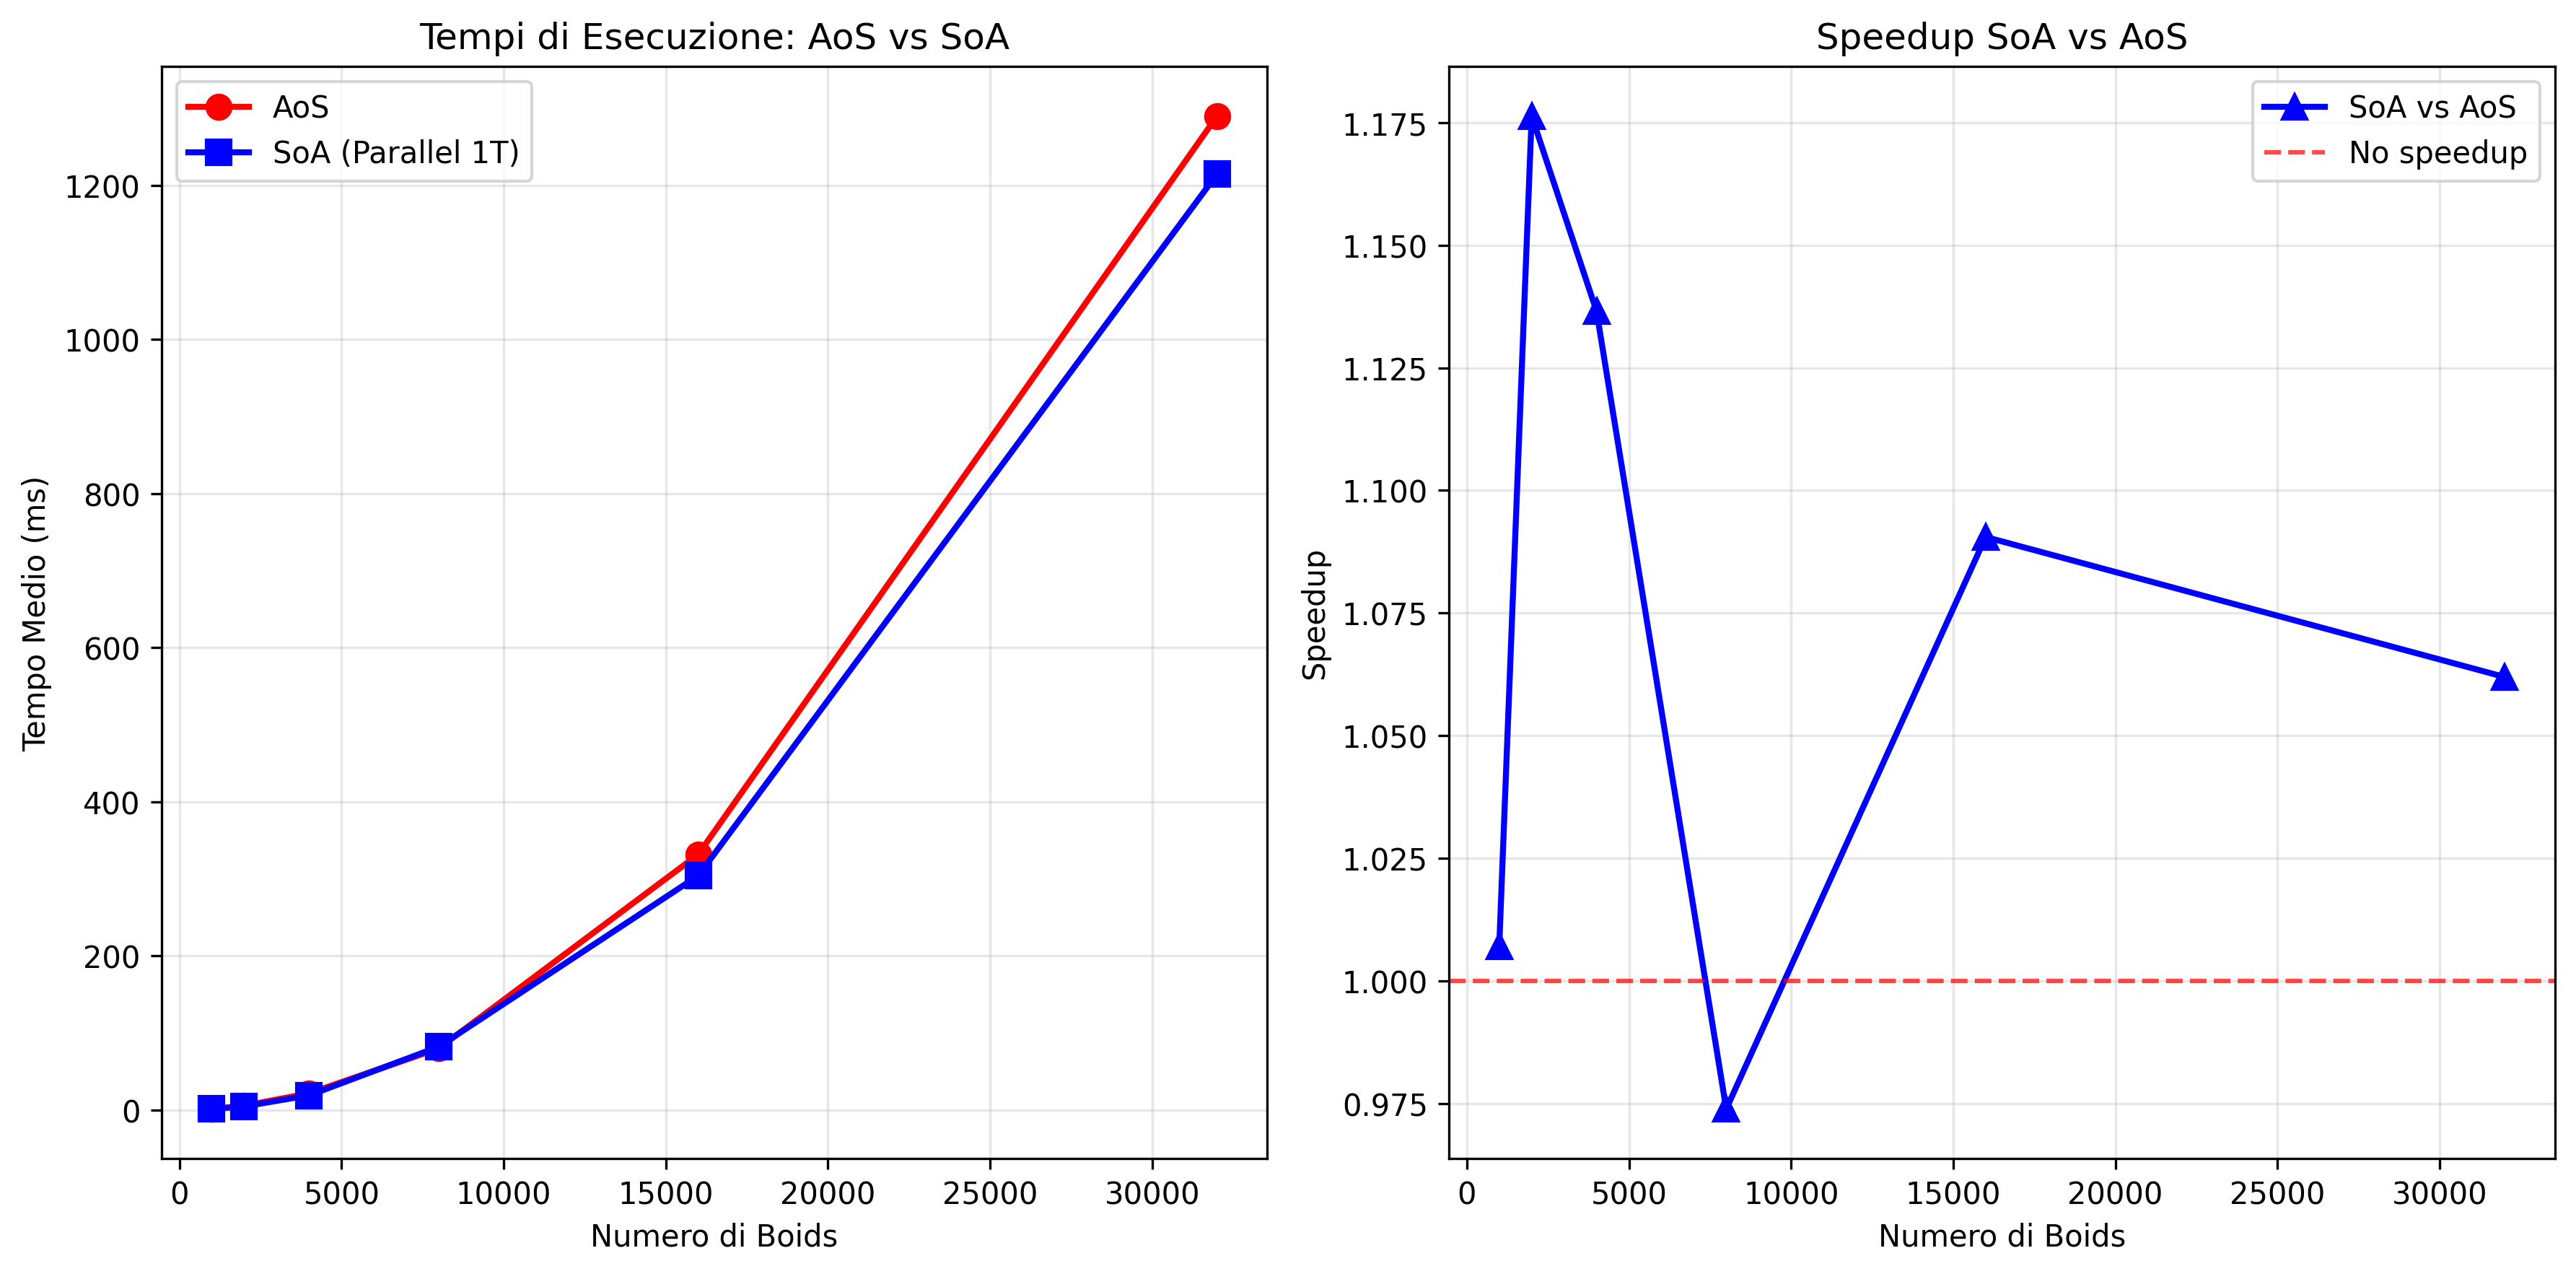
\includegraphics[width=0.95\textwidth]{../../images/aos_vs_soa.png}
\end{figure}

\textbf{Key Findings:}
\begin{itemize}
    \item SoA provides modest but consistent performance improvement
    \item 6.2\% improvement for 32,000 boids (1,290.09ms vs 1,214.82ms)
    \item Benefits become more pronounced with larger datasets
    \item Foundation for effective parallelization
\end{itemize}

\section{Parallel Scaling Performance}

\begin{figure}[h]
\centering
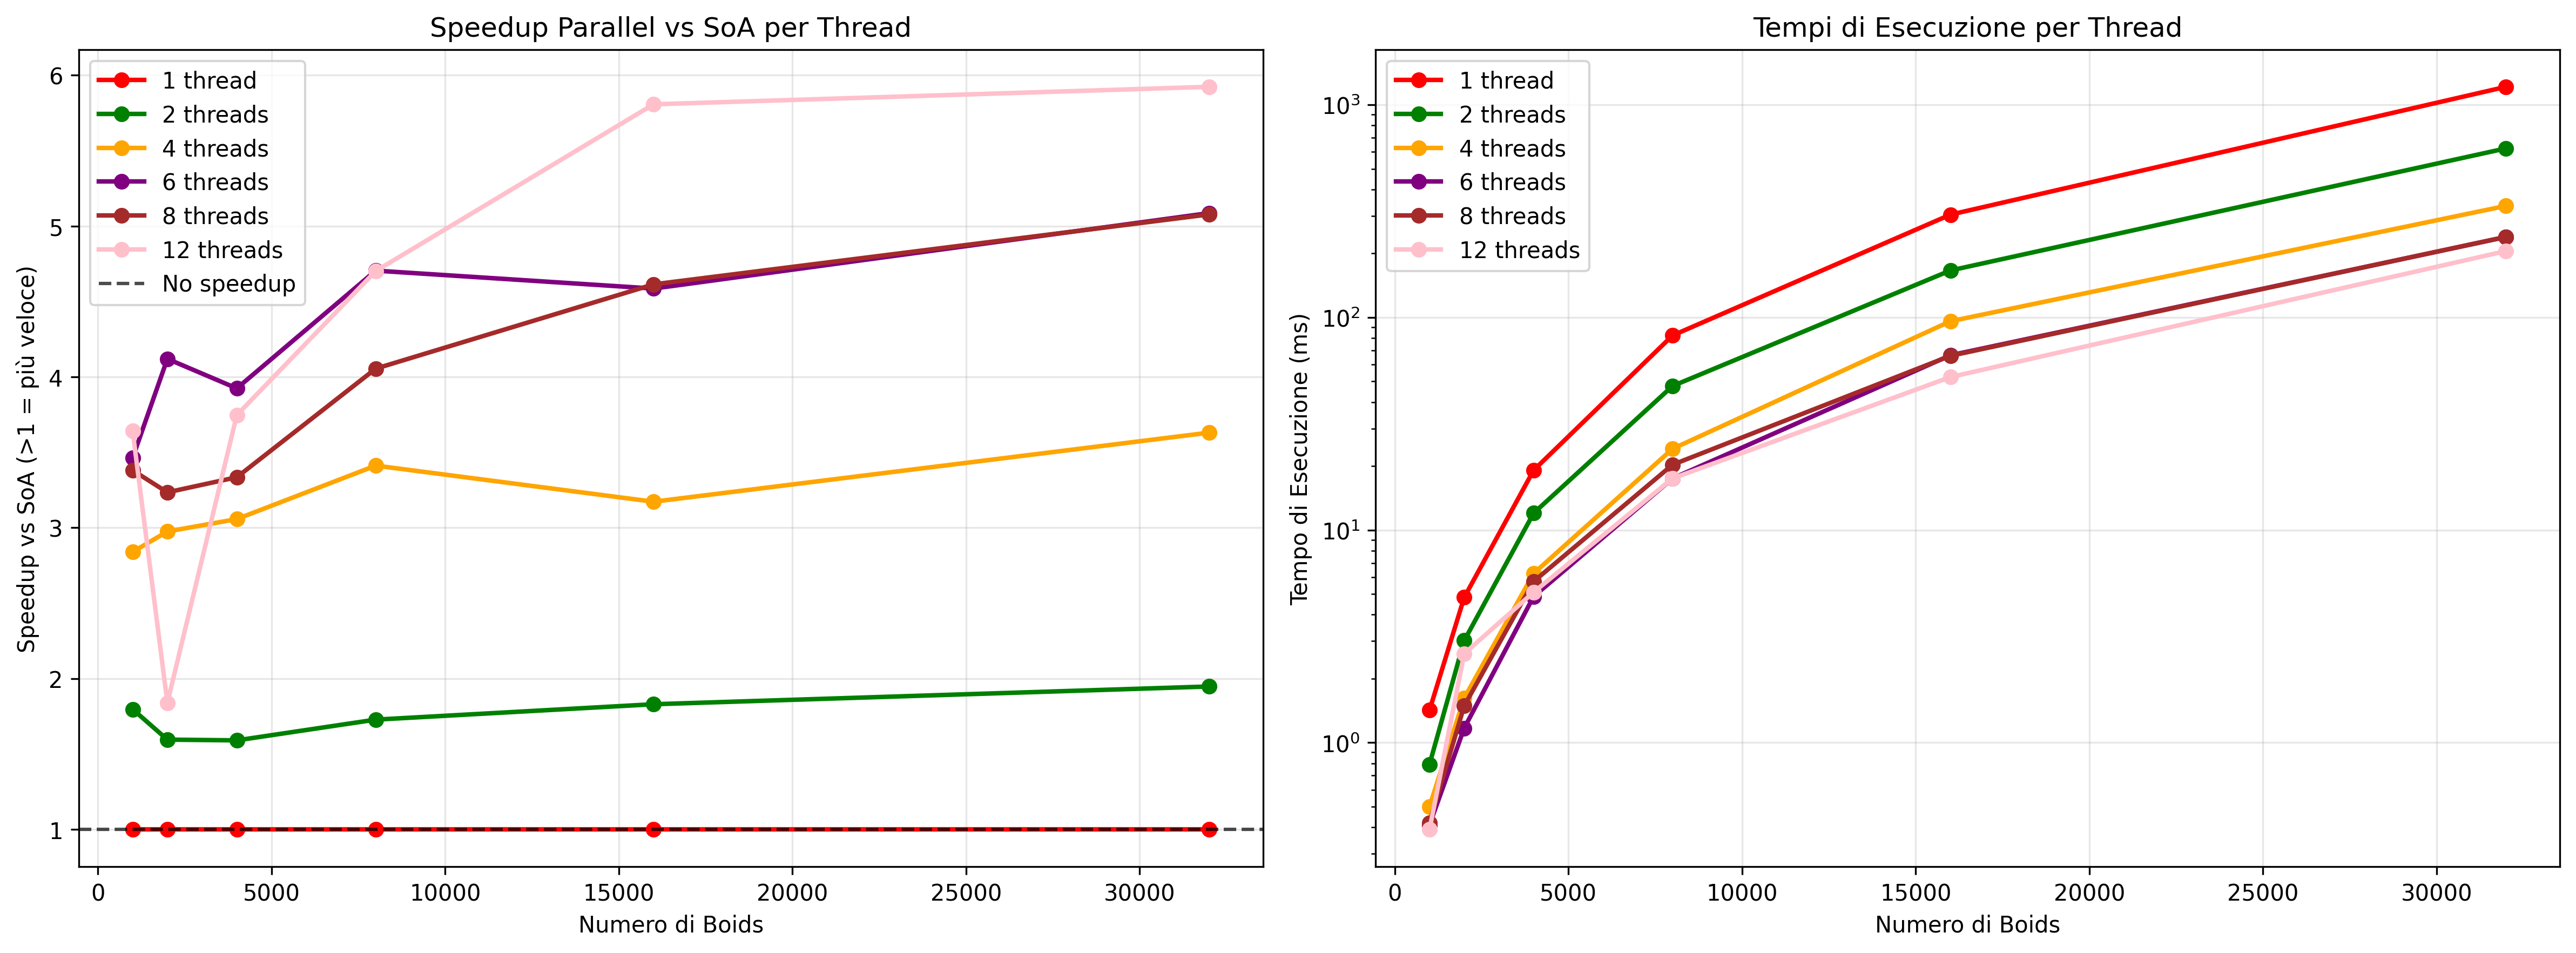
\includegraphics[width=1\textwidth]{../../images/parallel_analysis_performance.png}
\end{figure}

\newpage
\begin{center}
    \textbf{Speedup Results:}
    \begin{itemize}
        \item Near-linear scaling up to 6 threads
        \item Diminishing returns beyond 8-12 threads due to overhead
    \end{itemize}
    \begin{tabular}{|c|c|c|c|}
    \hline
    \textbf{Dataset Size} & \textbf{Sequential (ms)} & \textbf{Best Parallel (ms)} & \textbf{Speedup} \\
    \hline
    1,000 boids & 1.42 & 0.39 & 3.6x \\
    4,000 boids & 22.69 & 4.85 & 4.7x \\
    8,000 boids & 82.23 & 17.48 & 4.7x \\
    16,000 boids & 367.89 & 74.23 & 5.0x \\
    32,000 boids & 1,214.82 & 205.12 & 5.9x \\
    \hline
    \end{tabular}
\end{center}

\begin{figure}[h]
\centering
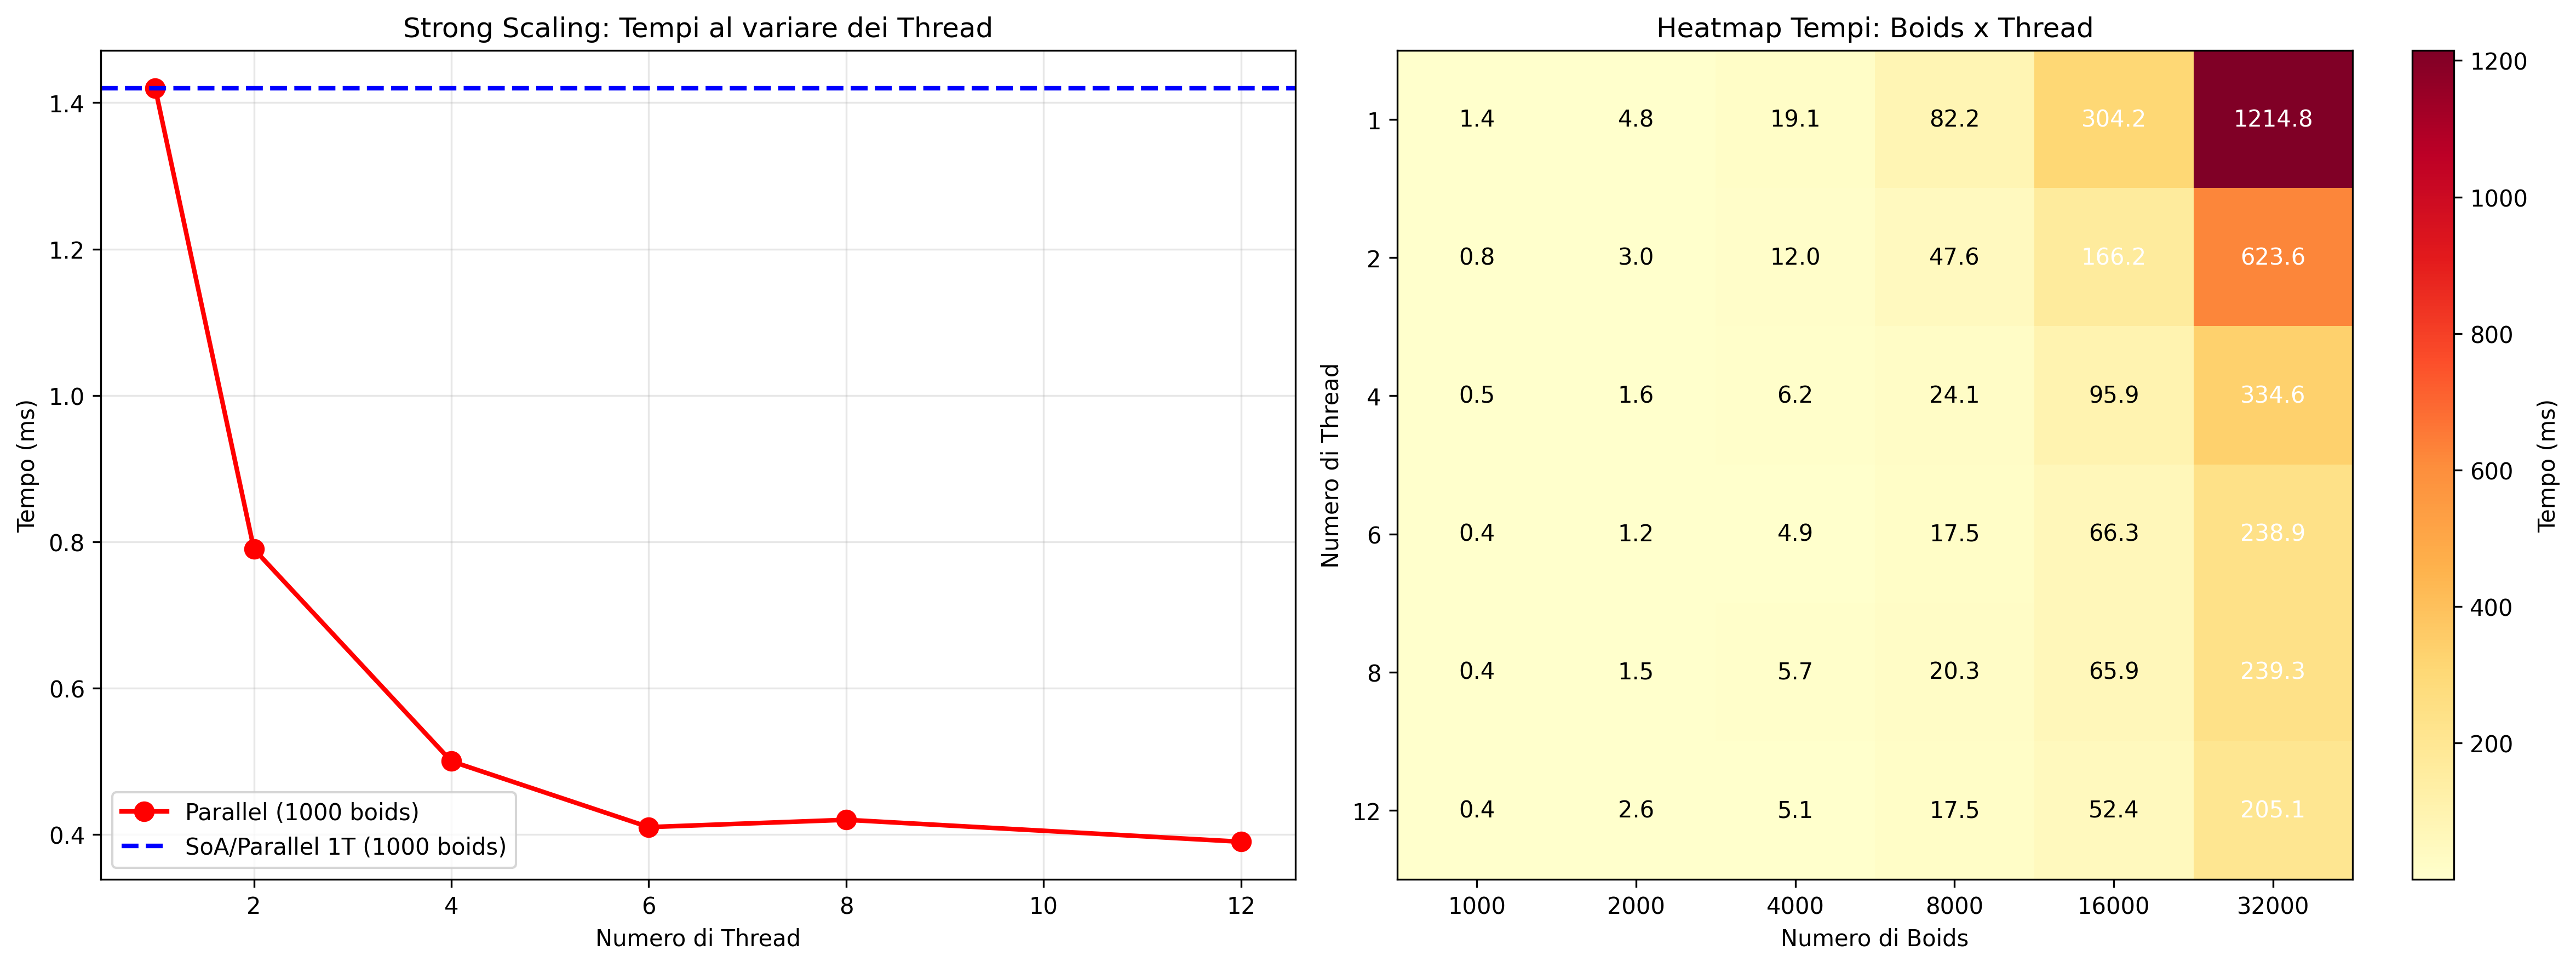
\includegraphics[width=0.95\textwidth]{../../images/parallel_analysis_scaling.png}
\end{figure}

\section{Conclusions}

\textbf{Project Achievements:}
\begin{itemize}
    \item Successfully implemented and optimized Boids simulation
    \item Demonstrated significant performance improvements through parallelization
    \item Validated importance of data structure optimization
    \item Achieved up to 5.9x speedup on multi-core systems
\end{itemize}